%%%%%%%%%%%%%%%%%%%%%%%%%%%%%%%%%%%%%%%%%
% Beamer Presentation
% LaTeX Template
% Version 1.0 (10/11/12)
%
% This template has been downloaded from:
% http://www.LaTeXTemplates.com
%
% License:
% CC BY-NC-SA 3.0 (http://creativecommons.org/licenses/by-nc-sa/3.0/)
%
%%%%%%%%%%%%%%%%%%%%%%%%%%%%%%%%%%%%%%%%%

%----------------------------------------------------------------------------------------
%	PACKAGES AND THEMES
%----------------------------------------------------------------------------------------

\documentclass{beamer}
\usepackage{subcaption}


\mode<presentation> {

% The Beamer class comes with a number of default slide themes
% which change the colors and layouts of slides. Below this is a list
% of all the themes, uncomment each in turn to see what they look like.

\usetheme{default}
%\usetheme{AnnArbor}
%\usetheme{Antibes}
%\usetheme{Bergen}
%\usetheme{Berkeley}
%\usetheme{Berlin}
%\usetheme{Boadilla}
%\usetheme{CambridgeUS}
%\usetheme{Copenhagen}
%\usetheme{Darmstadt}
%\usetheme{Dresden}
%\usetheme{Frankfurt}
%\usetheme{Goettingen}
%\usetheme{Hannover}
%\usetheme{Ilmenau}
%\usetheme{JuanLesPins}
%\usetheme{Luebeck}
%\usetheme{Madrid}
%\usetheme{Malmoe}
%\usetheme{Marburg}
%\usetheme{Montpellier}
%\usetheme{PaloAlto}
%\usetheme{Pittsburgh}
%\usetheme{Rochester}
%\usetheme{Singapore}
%\usetheme{Szeged}
%\usetheme{Warsaw}

% As well as themes, the Beamer class has a number of color themes
% for any slide theme. Uncomment each of these in turn to see how it
% changes the colors of your current slide theme.

%\usecolortheme{albatross}
%\usecolortheme{beaver}
%\usecolortheme{beetle}
%\usecolortheme{crane}
%\usecolortheme{dolphin}
%\usecolortheme{dove}
%\usecolortheme{fly}
%\usecolortheme{lily}
%\usecolortheme{orchid}
%\usecolortheme{rose}
%\usecolortheme{seagull}
%\usecolortheme{seahorse}
%\usecolortheme{whale}
%\usecolortheme{wolverine}

%\setbeamertemplate{footline} % To remove the footer line in all slides uncomment this line
%\setbeamertemplate{footline}[page number] % To replace the footer line in all slides with a simple slide count uncomment this line

%\setbeamertemplate{navigation symbols}{} % To remove the navigation symbols from the bottom of all slides uncomment this line
}

\usepackage{graphicx} % Allows including images
\usepackage{booktabs} % Allows the use of \toprule, \midrule and \bottomrule in tables
\usepackage{amsmath}
\usepackage{amsthm}
\usepackage{amssymb}
\usepackage{graphicx}
\usepackage[numbers]{natbib}


\global\long\def\argmin{\operatornamewithlimits{argmin}}
\global\long\def\argmax{\operatornamewithlimits{argmax}}

\theoremstyle{plain}
\newtheorem{thm}{\protect\theoremname}
  \theoremstyle{definition}
  \newtheorem{condition}{\protect\conditionname}
  \theoremstyle{plain}
  \newtheorem{prop}{\protect\propositionname}
  \theoremstyle{plain}
  \newtheorem{lem}{\protect\lemmaname}
\makeatother

  \providecommand{\conditionname}{Condition}
  \providecommand{\lemmaname}{Lemma}
  \providecommand{\propositionname}{Proposition}
\providecommand{\theoremname}{Theorem}

%----------------------------------------------------------------------------------------
%	TITLE PAGE
%----------------------------------------------------------------------------------------

\title[Short title]{{\Huge{Manifold Learning for Image Processing}} \\ .............................................................................\\} % The short title appears at the bottom of every slide, the full title is only on the title page

\author{Pankaj Kumar} % Your name
\institute[MIPT] % Your institution as it will appear on the bottom of every slide, may be shorthand to save space
{
Moscow Institute of Physics and Technology\\ % Your institution for the title page
\medskip
\textit{kumar.x.pankaj@gmail.com} % Your email address
}
\date{\today} % Date, can be changed to a custom date

\begin{document}

\begin{frame}
\titlepage % Print the title page as the first slide
\end{frame}

\begin{frame}
\frametitle{Overview} % Table of contents slide, comment this block out to remove it
\tableofcontents % Throughout your presentation, if you choose to use \section{} and \subsection{} commands, these will automatically be printed on this slide as an overview of your presentation
\end{frame}

%----------------------------------------------------------------------------------------
%	PRESENTATION SLIDES
%----------------------------------------------------------------------------------------
\section{Introduction}
\begin{frame}{Introduction}
\begin{itemize}
\item Data is everywhere
\item Data is being recorded at an unprecedented rate.
\item How do we find out the useful information?

\end{itemize}

\begin{figure}[!htb]
\minipage{0.32\textwidth}
  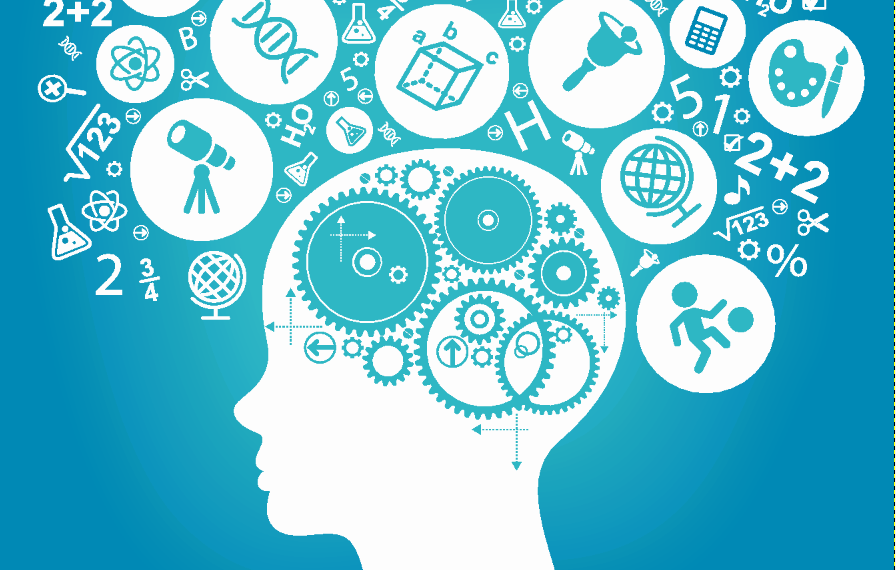
\includegraphics[height=3cm,width=3cm]{./figures/I_1.png}
%\caption{}\label{fig:awesome_image1} 
\endminipage\hfill
\minipage{0.32\textwidth}
  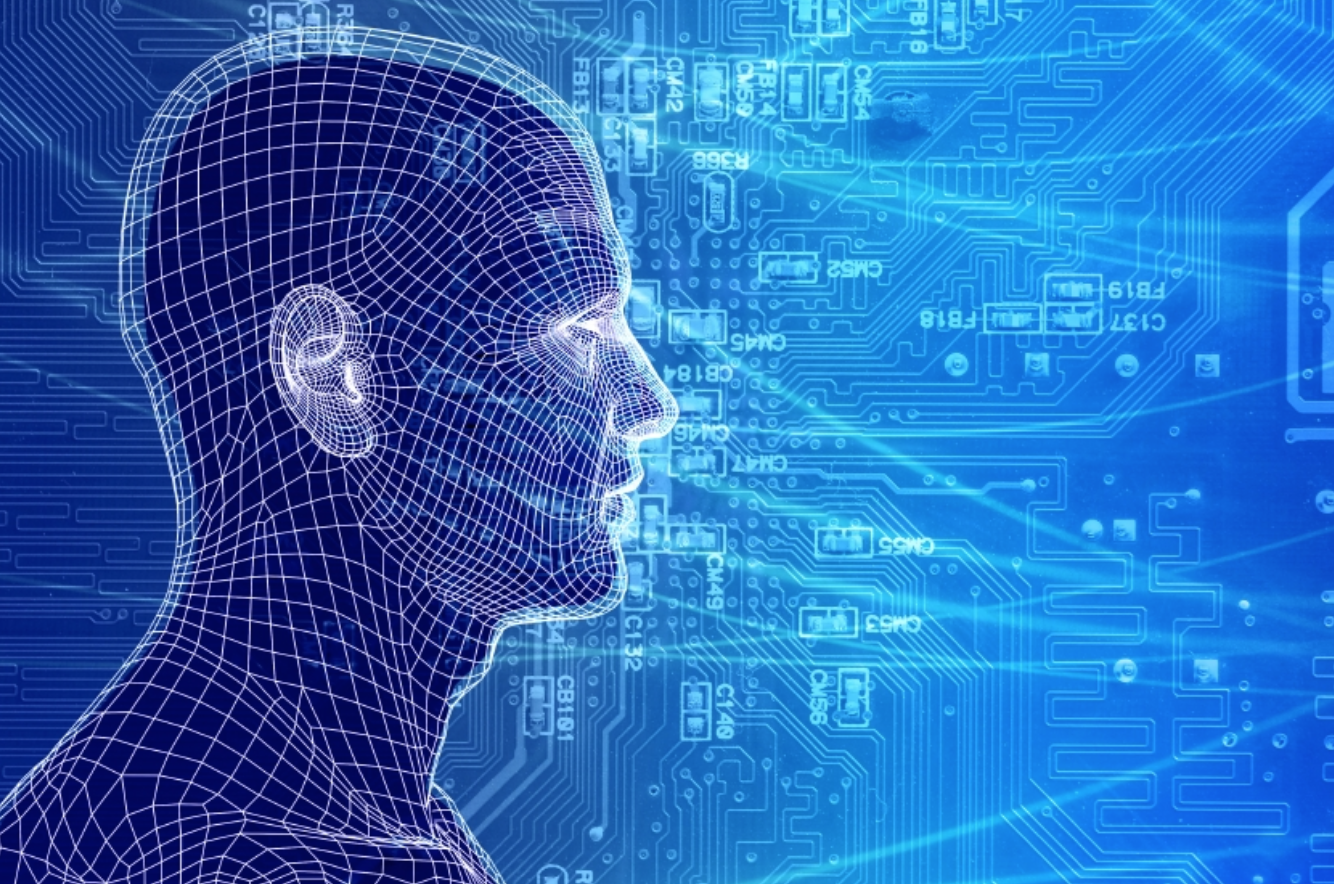
\includegraphics[height=3cm,width=3cm]{./figures/I_2.png}
% \caption{}\label{fig:awesome_image2}
\endminipage\hfill
\minipage{0.32\textwidth}%
  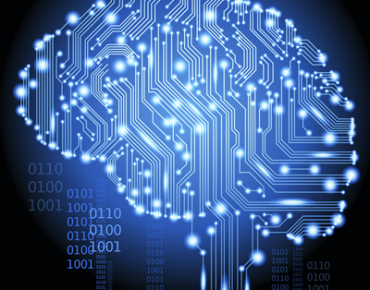
\includegraphics[height=3cm,width=3cm]{./figures/I_3.png}
% \caption{}\label{fig:awesome_image3}
\endminipage
\end{figure}

\pause

\begin{itemize}
\item By effective modeling of high-dimensional observed data, such that it capture the structure of the information content in a concise manner.
\end{itemize}

\end{frame}
%----------------------------------------------------------------------------
\begin{frame}{Image Processing}
\begin{itemize}
\item Digital revolution have infused enormous amount of images and video, which is growing constantly.
\item Each image sequence is a point in a space of dimension equal to the number of image pixels.
\item So the observation space is of possibly thousands/millions of dimensions.
\item The data is embedded as sub-manifold in high dimensional space.
\item Learning this manifold is a natural approach to the problem of manifold learning algorithms.
\end{itemize}

\end{frame}
%----------------------------------------------------------------------------
\section{Manifold Learning}
\begin{frame}{Manifold Learning}
Manifold learning is form of unsupervised machine learning algorithms, which  extract low-dimensional structure from high dimensional data. 

It can be further illustrated in below figure, where manifold learning algorithms for non-linear data builds an embedding function $f$ mapping $\mathcal{M}$ to $\mathbb{R}^2$.

\begin{figure}[ht]
\begin{center}
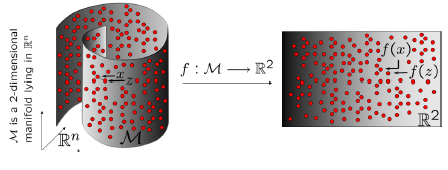
\includegraphics[width=\textwidth]{./Figures/manifold.png}
%\caption{Manifold Learning}
%\label{fig:manifold}
\end{center}
\end{figure}
\end{frame}

%----------------------------------------------------------------------------
\subsection{Problem Definition}
\begin{frame}{Problem}
Given a set of of high-dimensional training instances $\mathbb{X} = \{x_1, x_2, ...,x_N \}$, where $x_{i} \in \mathbb{R}^D$. We assume that $\mathbb{X}$ approximately lie on a smooth manifold $\mathcal{X}$. The idea of manifold learning algorithms is to find an embedding set $\mathbb{Y} = \{y_1, y_2, ...,y_N \} $ of $\mathbb{X}$ in low dimension space $\mathbb{R}^d$, where $d<D$. The local manifold structure formed by $\mathbb{X}$ in the original space $\mathbb{R}^D$ is preserved in the embedded space $\mathbb{R}^d$.
\end{frame}
%---------------------------------------------------------------------------
\subsection{Linear Methods}
\begin{frame}{Linear Methods}
\begin{itemize}
\item Principal Components Analysis (PCA)
\item Metric Multidimensional Scaling (MDS)
\end{itemize}
\end{frame}
%---------------------------------------------------------------------------
\begin{frame}{Principal Components Analysis (PCA)}
\begin{figure}[ht]
\begin{center}
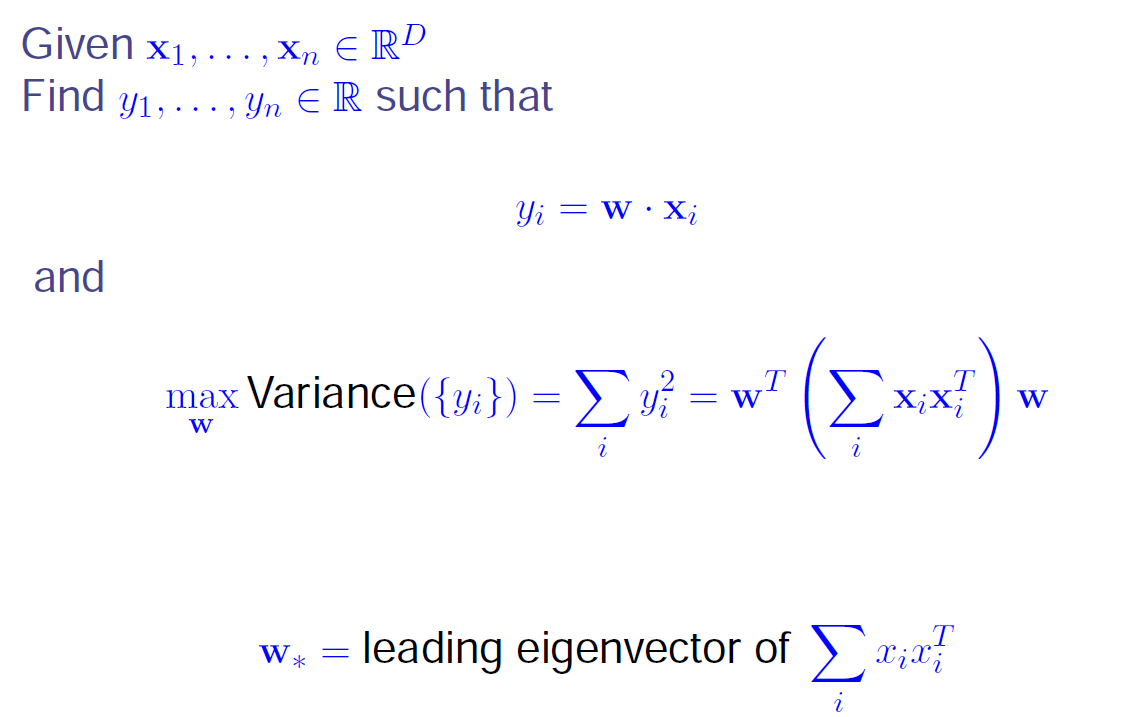
\includegraphics[width=\textwidth]{./figures/PCA.png}
%\caption{Manifold Learning}
%\label{fig:manifold}
\end{center}
\end{figure}

\end{frame}
%---------------------------------------------------------------------------

\begin{frame}{Metric Multidimensional Scaling (MDS)}
\begin{figure}[ht]
\begin{center}
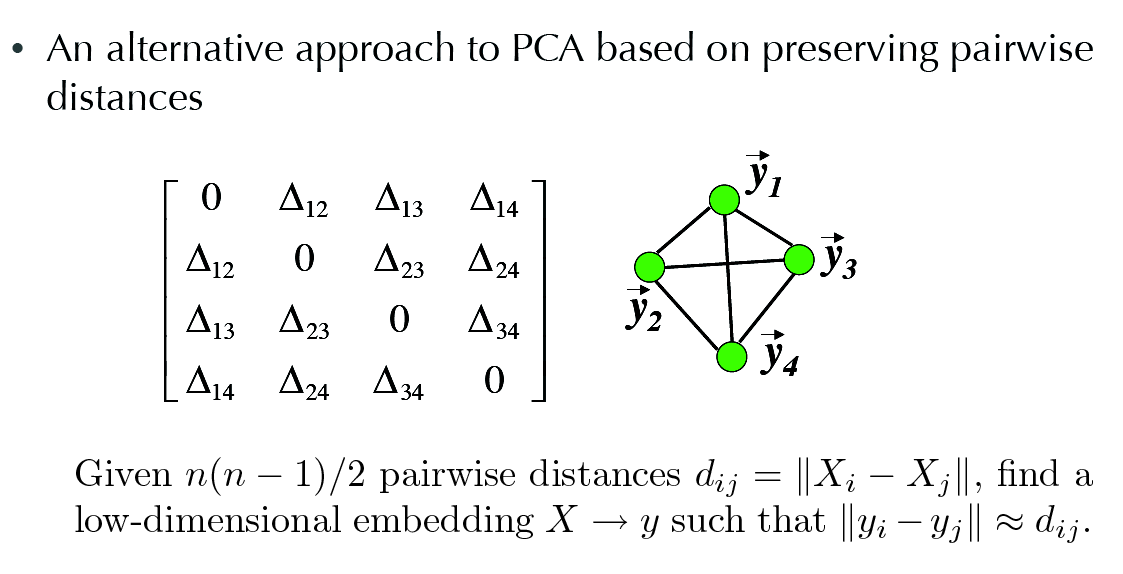
\includegraphics[width=\textwidth]{./figures/MDS.png}
%\caption{Manifold Learning}
%\label{fig:manifold}
\end{center}
\end{figure}

\end{frame}
%---------------------------------------------------------------------------
\subsection{Non-Linear Methods}
\begin{frame}{Non-Linear Methods}
\begin{itemize}
\item Isomap
\item Locally Linear Embedding
\item Laplacian Eigenmaps
\item Diffusion Maps
\item Hessian eigenmaps
\item Local Tangent Space Alignment
\end{itemize}

\end{frame}
%---------------------------------------------------------------------------
\begin{frame}{Isomap}
\begin{figure}[ht]
\begin{center}
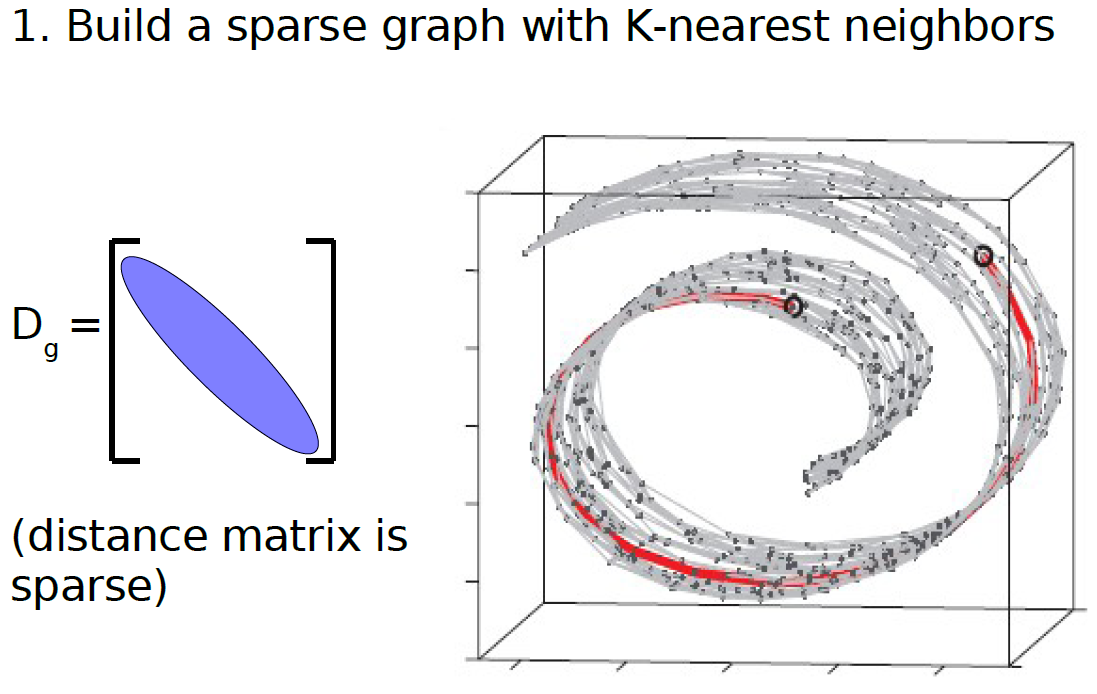
\includegraphics[width=\textwidth]{./figures/ISO_1.png}
%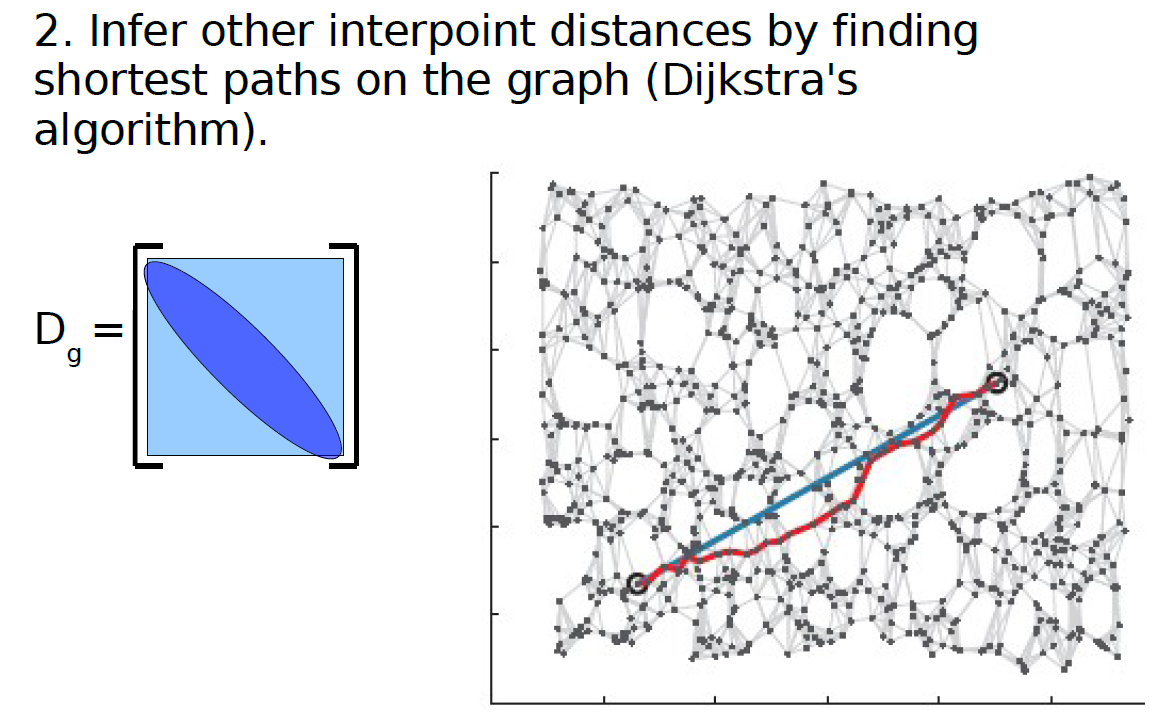
\includegraphics[width=\textwidth]{./figures/ISO_2.png}
%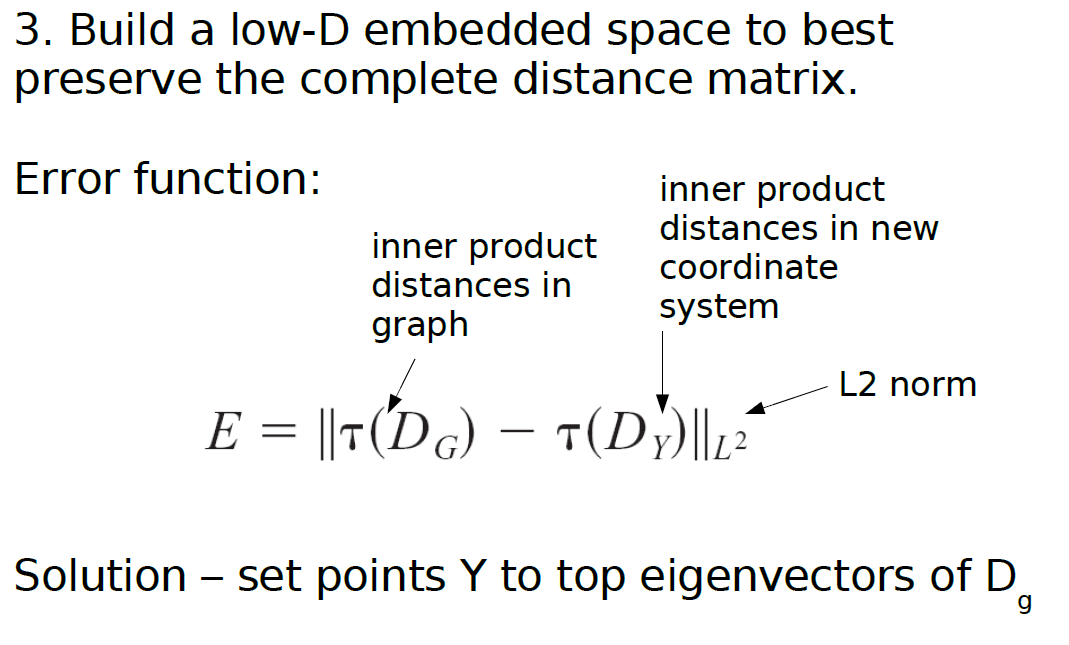
\includegraphics[width=\textwidth]{./figures/ISO_3.png}
%\caption{Manifold Learning}
%\label{fig:manifold}
\end{center}
\end{figure}
\end{frame}
%----------------------------------------------------------------------------
\begin{frame}{Isomap}
\begin{figure}[ht]
\begin{center}
%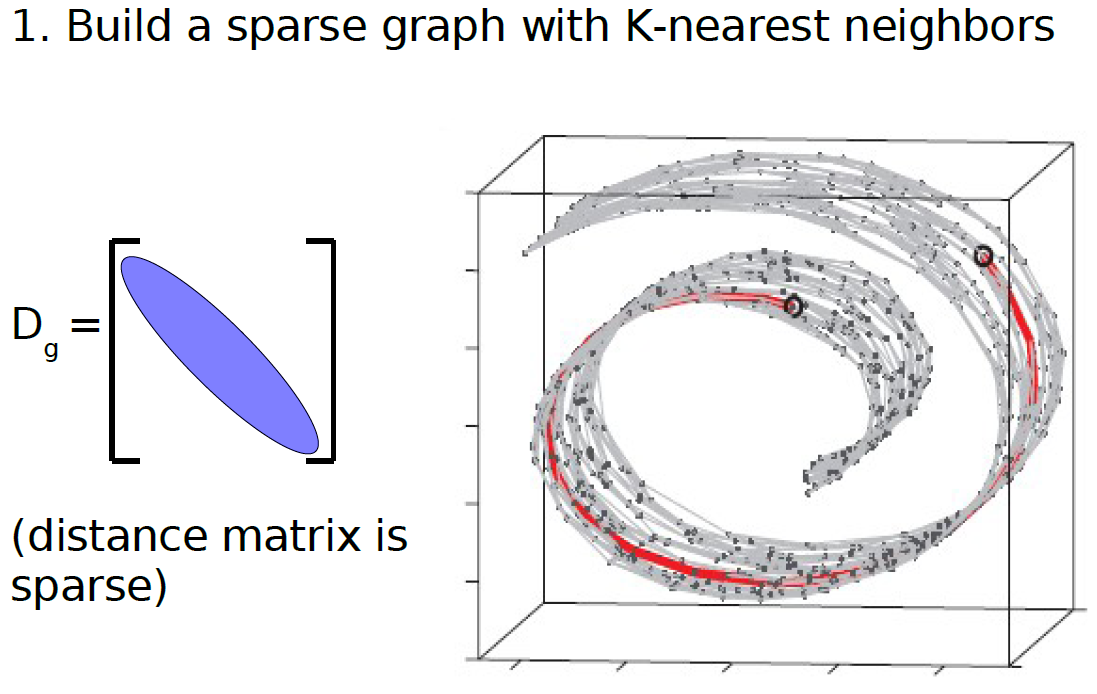
\includegraphics[width=\textwidth]{./figures/ISO_1.png}
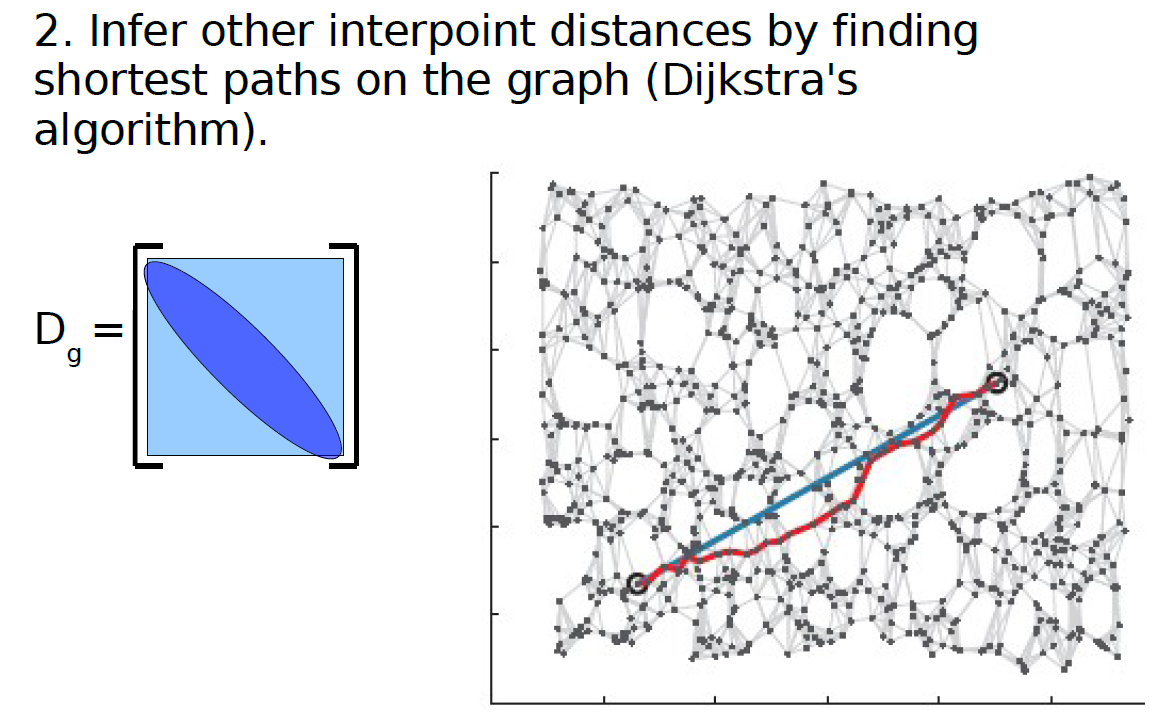
\includegraphics[width=\textwidth]{./figures/ISO_2.png}
%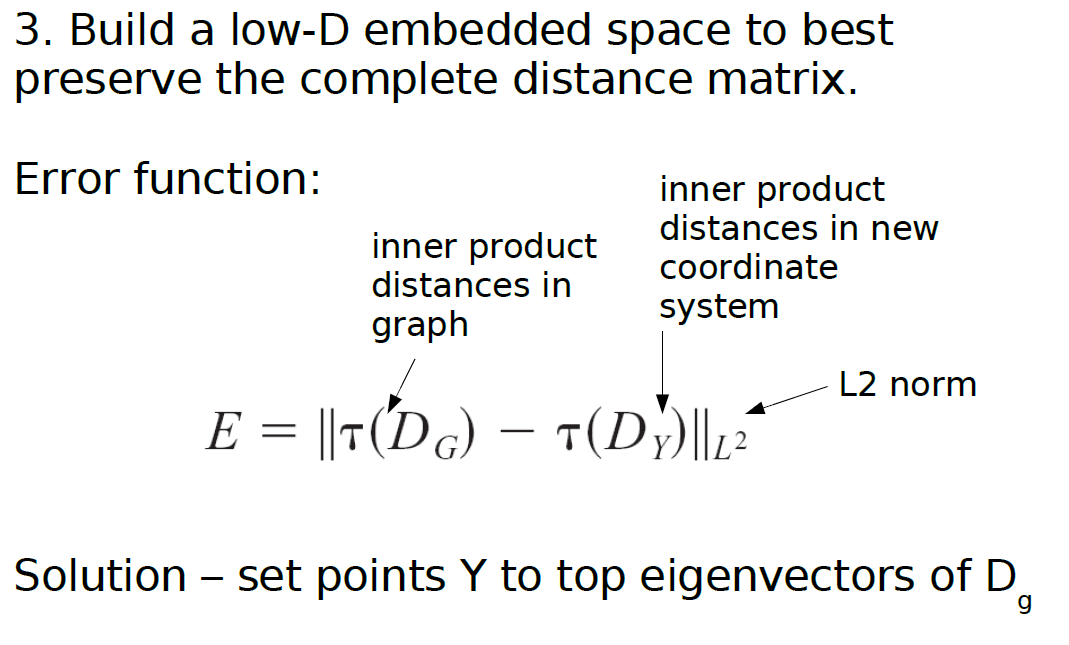
\includegraphics[width=\textwidth]{./figures/ISO_3.png}
%\caption{Manifold Learning}
%\label{fig:manifold}
\end{center}
\end{figure}
\end{frame}
%---------------------------------------------------------------------------
\begin{frame}{Isomap}
\begin{figure}[ht]
\begin{center}
%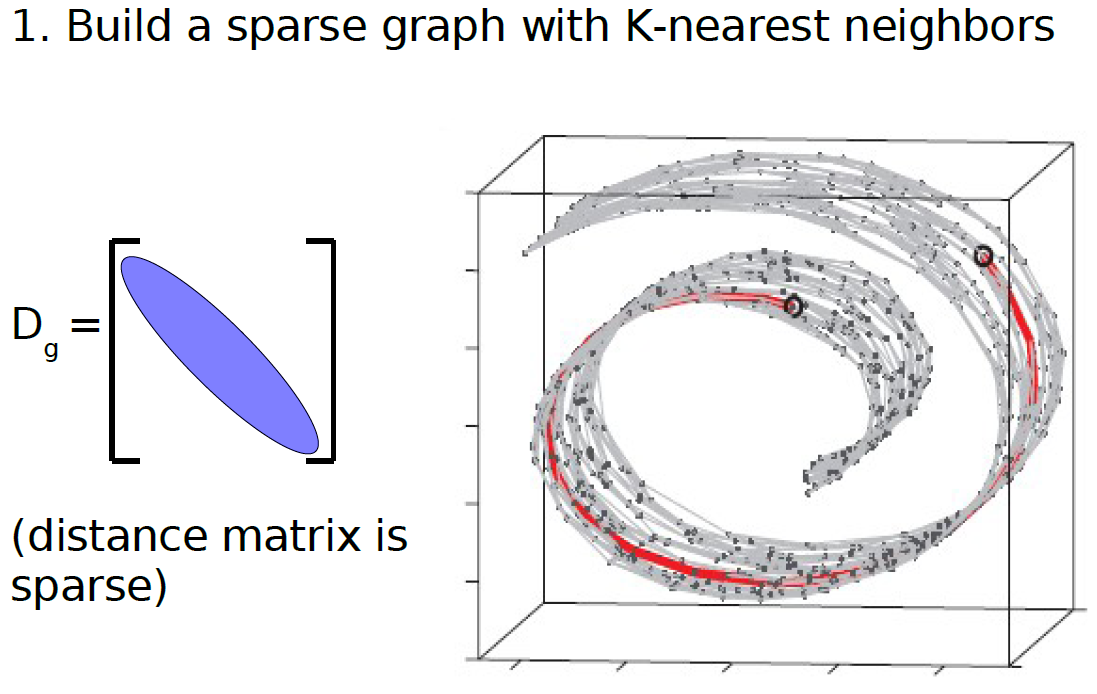
\includegraphics[width=\textwidth]{./figures/ISO_1.png}
%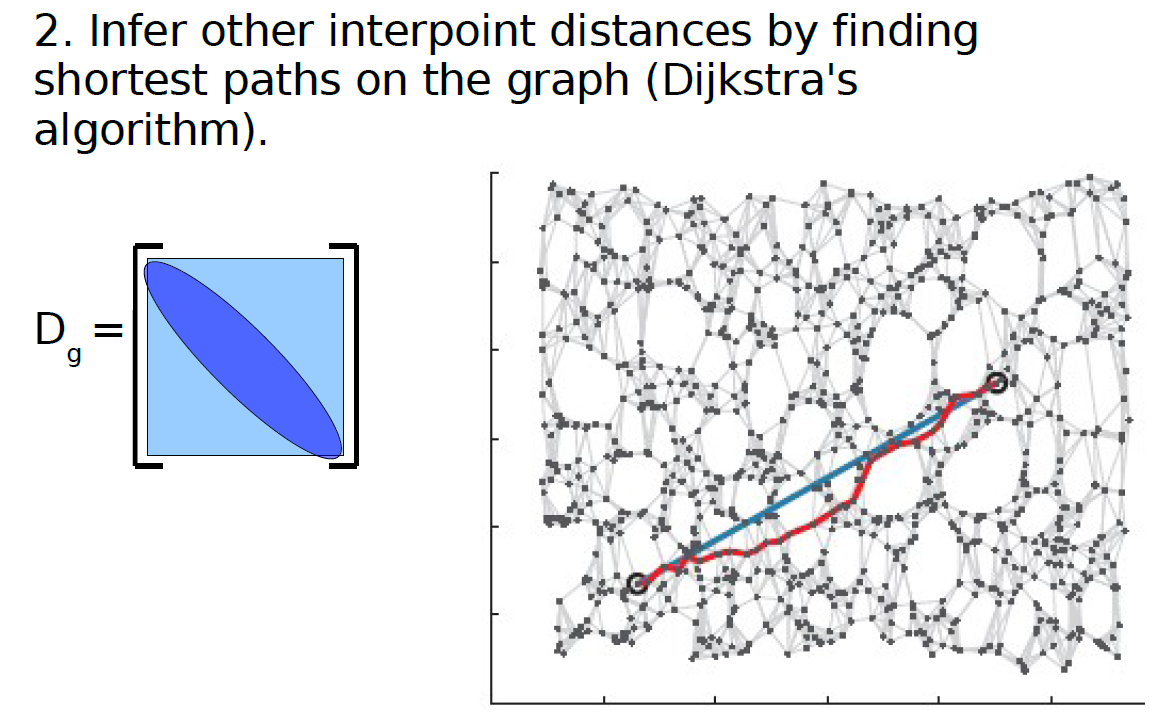
\includegraphics[width=\textwidth]{./figures/ISO_2.png}
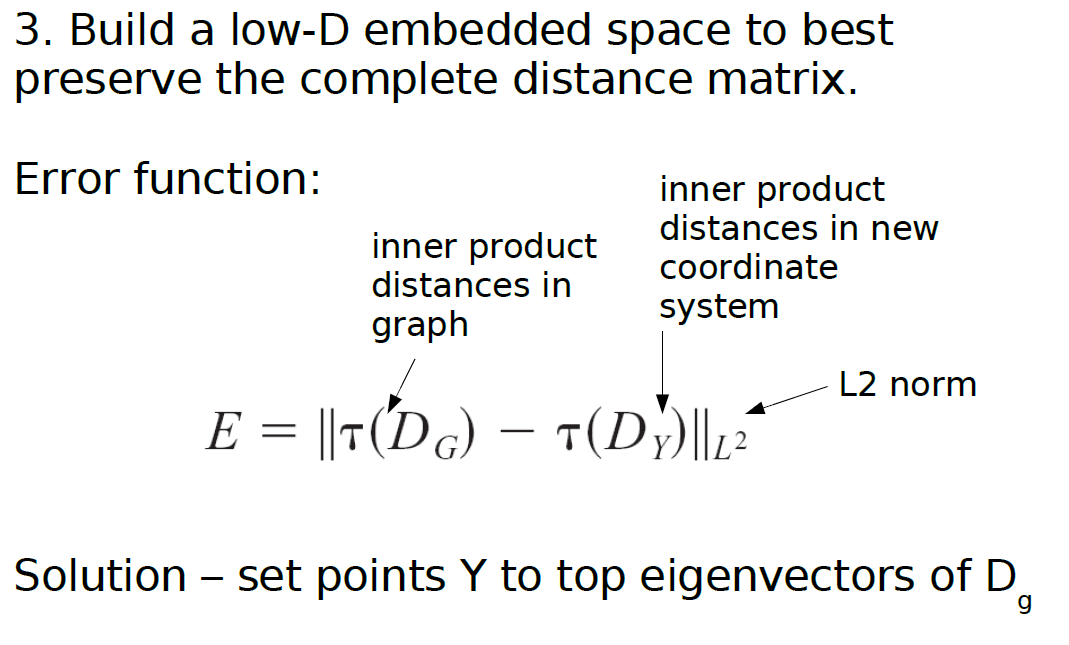
\includegraphics[width=\textwidth]{./figures/ISO_3.png}
%\caption{Manifold Learning}
%\label{fig:manifold}
\end{center}
\end{figure}
\end{frame}
%---------------------------------------------------------------------------
\begin{frame}{Locally Linear Embedding}
\begin{figure}[ht]
\begin{center}
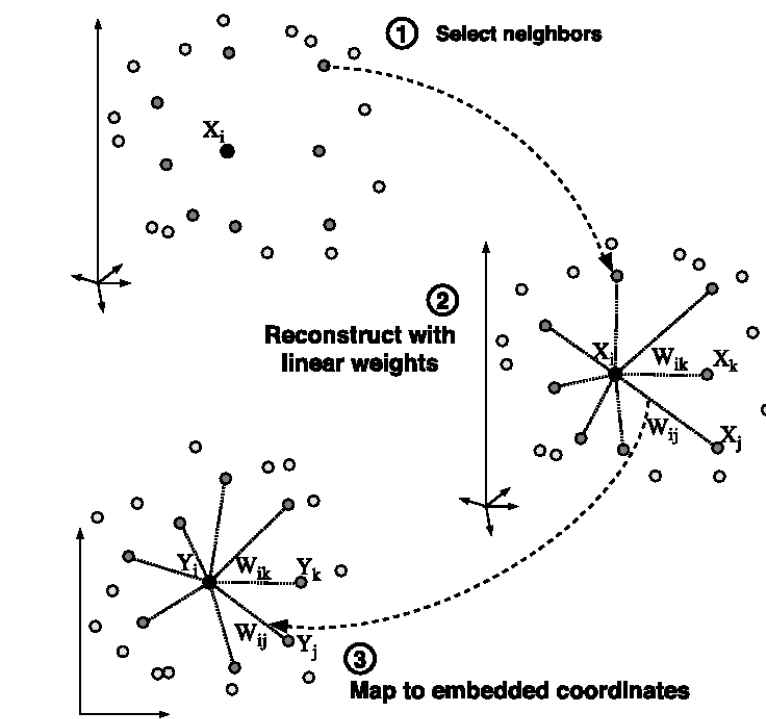
\includegraphics[width=8cm, height=8cm]{./figures/LLE.png}
%\caption{Manifold Learning}
%\label{fig:manifold}
\end{center}
\end{figure}
\end{frame}
%---------------------------------------------------------------------------
\section{Contribution}
\begin{frame}{Contribution}
\begin{enumerate}
\item The research exploring the comparison of manifold learning algorithms is quite shallow. There are few theoretical comparisons results for these algorithms, but the primary evaluation methodology has been to run the
algorithm on artificial data sets and do comparison. We use MNIST datasets with optical character recognition in mind to evaluate the performance of the manifold learning algorithms.

\item Motivated by recent study, we presents a novel manifold learning approach for high dimensional data, with emphasis on the problem of anomaly detection in image.
\end{enumerate}


\end{frame}
%---------------------------------------------------------------------------
\section{Optical Character Recognition}
\subsection{Introduction}{Introduction}
\begin{frame}{Introduction}
\begin{itemize}
\item optical character recognition have found applications in bank check processing, assistive technology for visually impaired users, automatic number plate recognition and many more
\item A basic requirement for credibility of classification algorithms  requires a high accuracy on MNIST datasets, a hello world datasets.
\item The earlier experimental results doing comparison between different manifold learning algorithms show that these methods can work pretty well at least in our toy examples.
\end{itemize}
\end{frame}

%-----------------------------------------------------------------------------
\subsection{Data}
\begin{frame}{Data}
\begin{itemize}
\item The standardised MNIST database has a training set of 60,000 examples, and a test set of 10,000 examples.
\item Each example is of size $28\times28$, a total of 784 greyscale pixels.
\item Training set have 60,000 rows (images) and 785 (784 pixels and a one label) columns. 
\item Each row component contains a value between one and zero and this describes the intensity of each pixel.
\item Test set is same as training set, except no label and 10000 images.
\end{itemize}
\end{frame}
%---------------------------------------------------------------------------
\begin{frame}{First look}
\begin{figure}[h!]
\begin{center}
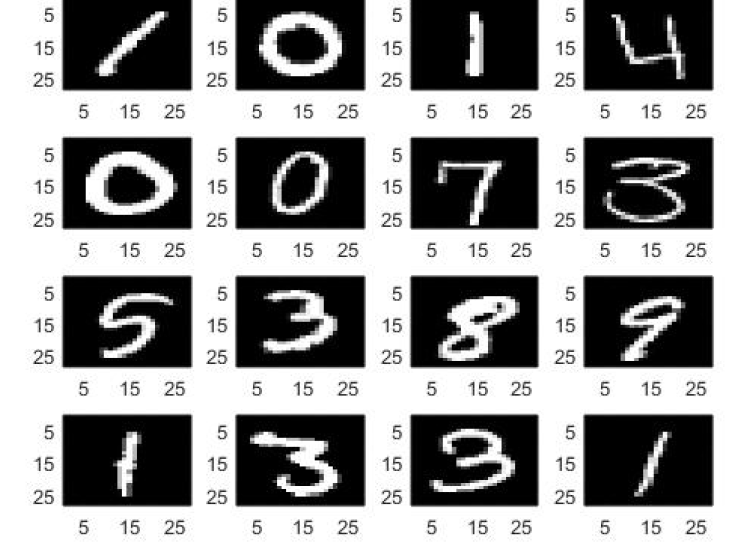
\includegraphics[width= 7cm, height =7cm]{./figures/O.png}
\caption {First look at MNIST data}
\label{4_1} 
\end{center}
\end{figure}
\end{frame}
%--------------------------------------------------------------------------
\subsection{Preprocessing}
\begin{frame}{Preprocessing: Hough transform}

\begin{figure}[h!]
\begin{center}
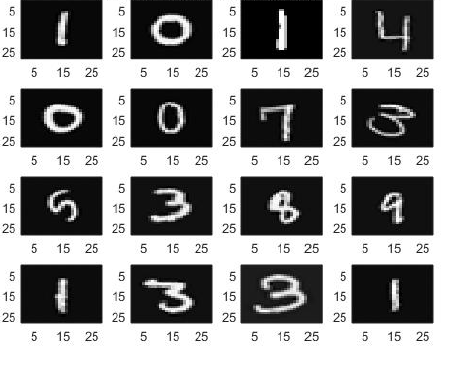
\includegraphics[width= 7cm, height =7cm]{./Figures/4_2.png}
\caption {Hough transform}
\label{4_2} 
\end{center}
\end{figure}

\end{frame}
%---------------------------------------------------------------------------
\subsection{Results and Discussion}
\begin{frame}{Pearson Correlation plot}
\begin{figure}[h!]
\begin{center}
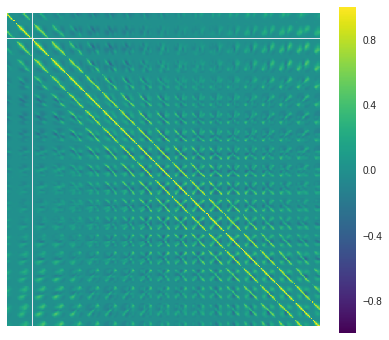
\includegraphics[width= 7cm, height =7cm]{./Figures/4_3.png}
\caption {Pearson Correlation plot 500 observations}
\label{4_3} 
\end{center}
\end{figure}
\end{frame}
%---------------------------------------------------------------------------
\subsubsection{Linear Method:PCA}
\begin{frame}{Explained Variance}
\begin{figure}[h!]
\begin{center}
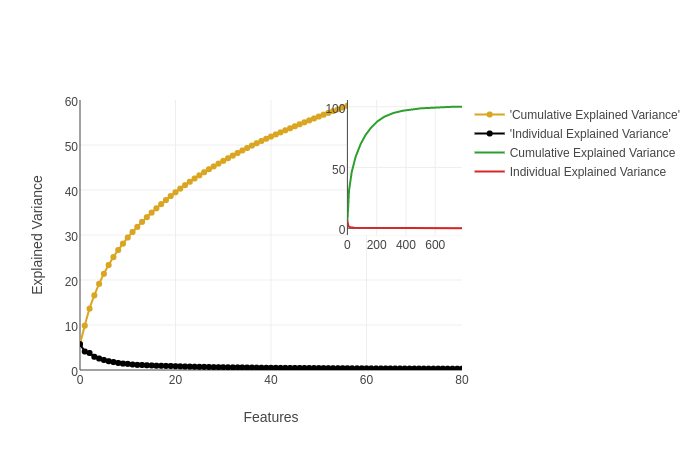
\includegraphics[width=\textwidth]{./Figures/pca_var.png}
\caption {Explained Variance}
\label{pca_var} 
\end{center}
\end{figure}
\end{frame}
%---------------------------------------------------------------------------
\begin{frame}{Eigenvalues}
\begin{figure}[h!]
\begin{center}
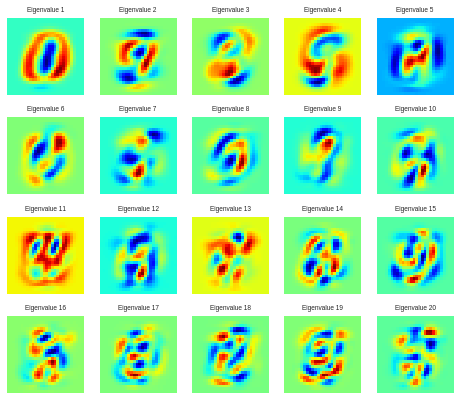
\includegraphics[width= 7cm, height =7cm]{./Figures/pca_vis.png}
\caption {Top 200 eigenvalues}
\label{pca_vis} 
\end{center}
\end{figure}
\end{frame}
%----------------------------------------------------------------------------
\begin{frame}{Digit Classification}
\begin{figure}[h!]
\begin{center}
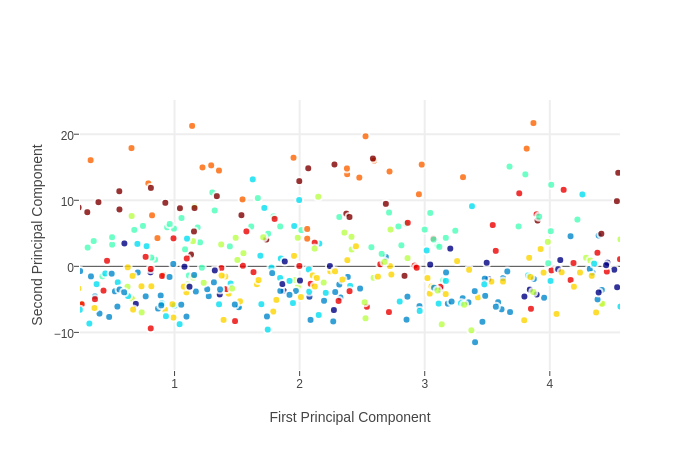
\includegraphics[width=\textwidth]{./Figures/pca_dr.png}
\caption {PCA}
\label{pca_dr} 
\end{center}
\end{figure}
\end{frame}
%---------------------------------------------------------------------------
\subsubsection{Non-Linear Method}

\begin{frame}{TSNE}
\begin{figure}[h!]
\begin{center}
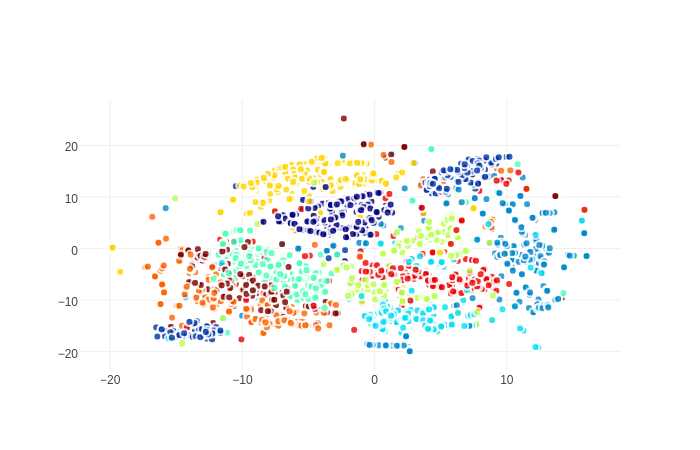
\includegraphics[width=\textwidth]{./Figures/tsne.png}
\caption {TSNE ( t-Distributed Stochastic Neighbour Embedding )}
\label{tsne} 
\end{center}
\end{figure}
\end{frame}
%---------------------------------------------------------------------------
\begin{frame}{Comparison: Manifold learning Algorithms}

\begin{figure}[h!]
\begin{center}
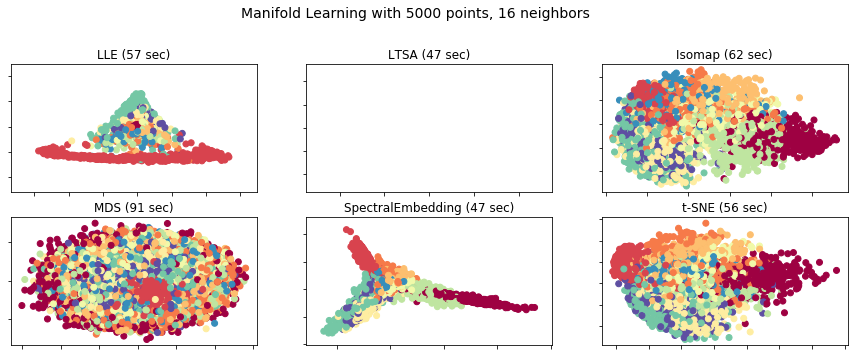
\includegraphics[width=\textwidth]{./Figures/AML.png}
\caption {Manifold Learning Algorithms Output}
\label{AML} 
\end{center}
\end{figure}
\end{frame}
%---------------------------------------------------------------------------
\begin{frame}{Out of sample}

\begin{figure}[t!] % "[t!]" placement specifier just for this example 
\begin{subfigure}{0.32\textwidth}
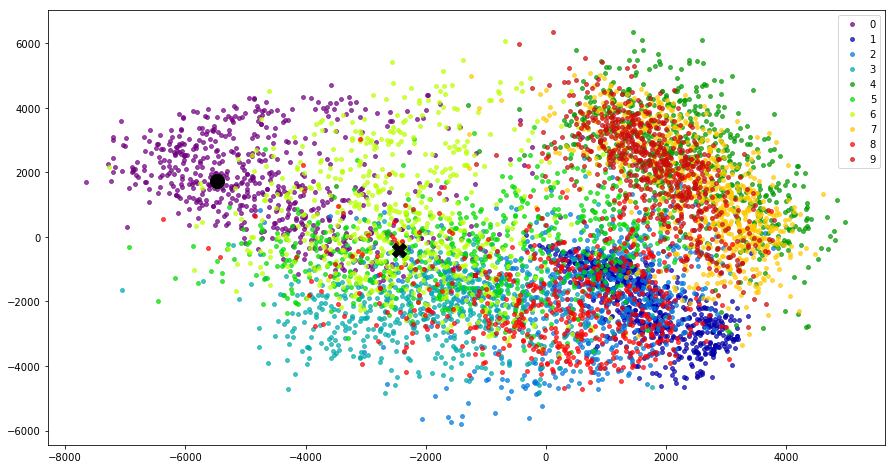
\includegraphics[height=3cm,width=4cm]{./Figures/LLE_OS.png}
\caption{LLE} 
\end{subfigure}\hspace*{\fill}
\begin{subfigure}{0.32\textwidth}
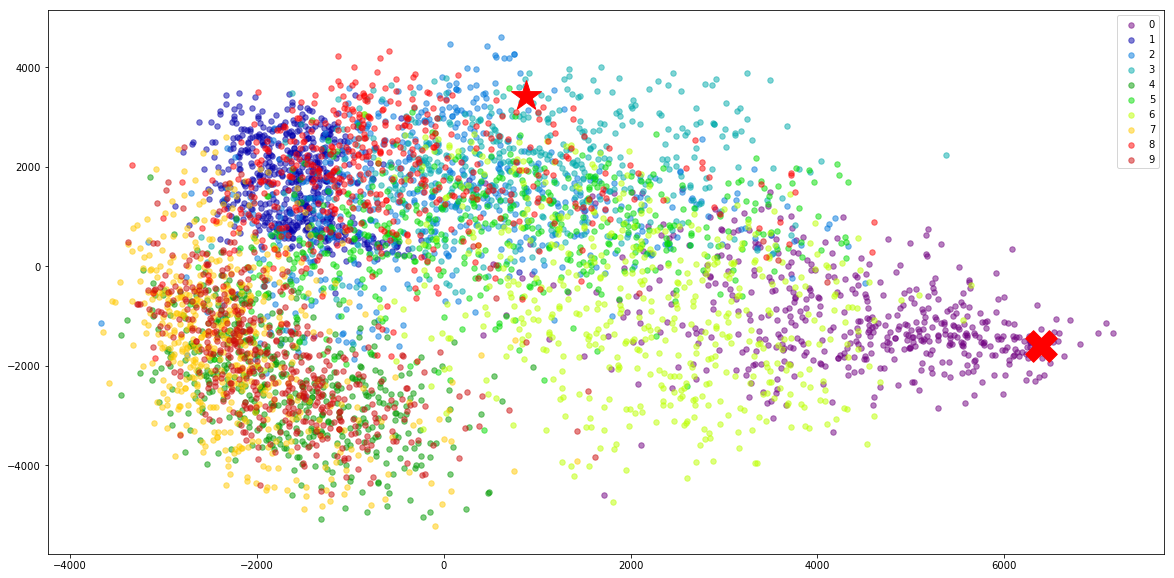
\includegraphics[height=3cm,width=4cm]{./Figures/ISO_OS.png}
\caption{ISOMAP} 
\end{subfigure}

\medskip
\begin{subfigure}{0.32\textwidth}
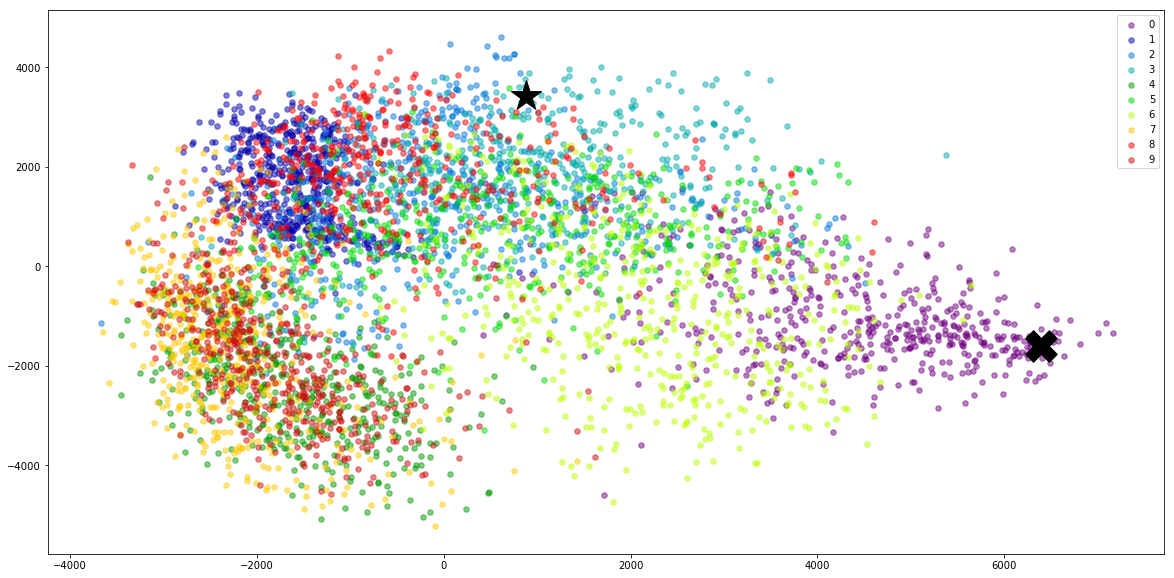
\includegraphics[height=3cm,width=4cm]{./Figures/SE_OS.png}
\caption{SE}
\end{subfigure}\hspace*{\fill}
\begin{subfigure}{0.32\textwidth}
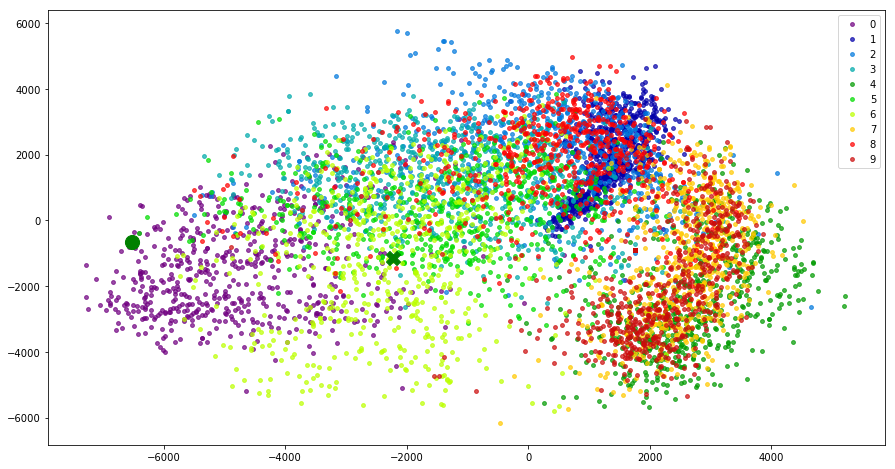
\includegraphics[height=3cm,width=4cm]{./Figures/TSNE_OS.png}
\caption{TSNE} 
\end{subfigure}

\caption{Out of sample predication for manifold learning algorithms} \label{OSML}
\end{figure}
\end{frame}
%---------------------------------------------------------------------------
\subsubsection{Recognition}
\begin{frame}{Models}
\begin{itemize}
\item To perform digit recognition task we used three supervised algorithms:  K-Nearest Neighbour (KNN) , Support Vector Machine (SVM)  and Convolutional Neural Networks (CNN).
\item By extracting n-components from the low dimension, we build train and text datasets corresponding to manifold learning algorithms. For example, $\mathbf{TEST}_{Isomap}$ and $\mathbf{Train}_{Isomap}$.
\item For dimension reduction, we take three manifold algorithms namely Isomap, Locally Linear Embedding and t-distributed Stochastic Neighbor Embedding.
\end{itemize}
\end{frame}
%---------------------------------------------------------------------------
\begin{frame}{Training}
\begin{itemize}
\item The 5-fold cross validation is performed on the training set comprising of original data and data created out of dimension reduction.
\item Then for every model, we choose the parameters yielding highest cross-validation classification accuracy.
\item  Finally, to obtain a real out of sample performance evaluation, we use the best model to predict on the test set.
\end{itemize}
\end{frame}
%---------------------------------------------------------------------------
\begin{frame}{Accuracy: Original}
\begin{table}[ht!]
\caption{Model Summary for $\mathbf{Data}$(original)}
% title of Table
\centering
% used for centering table
\begin{tabular}{c c c }
% centered columns (4 columns)
\hline\hline
%inserts double horizontal lines
Model & Data & Accuracy\\ [0.5ex]
% inserts table
%heading
\hline
% inserts single horizontal line
KNN & original& 91.00 \\
SVM & orignal & 95.60 \\
CNN & orignal & 93.00\\ [1ex]
% [1ex] adds vertical space
\hline
%inserts single line
\end{tabular}
\label{R:ORG}
% is used to refer this table in the text
\end{table}

\end{frame}
%---------------------------------------------------------------------------

\begin{frame}{Accuracy: Isomap}

\begin{table}[ht!]
\caption{Model Summary for $\mathbf{Data}$(isomap)}
% title of Table
\centering
% used for centering table
\begin{tabular}{c c c }
% centered columns (4 columns)
\hline\hline
%inserts double horizontal lines
Model & Data & Accuracy (\%)\\ [0.5ex]
% inserts table
%heading
\hline
% inserts single horizontal line
KNN & isomap & 92.00 \\
SVM & isomap & 95.50 \\
CNN & isomap & 93.00\\ [1ex]
% [1ex] adds vertical space
\hline
%inserts single line
\end{tabular}
\label{R:ISO}
% is used to refer this table in the text
\end{table}

\end{frame}
%---------------------------------------------------------------------------
\begin{frame}{Accuracy: TSNE}

\begin{table}[ht]
\caption{Model Summary for $\mathbf{Data}$(tsne)}
% title of Table
\centering
% used for centering table
\begin{tabular}{c c c }
% centered columns (4 columns)
\hline\hline
%inserts double horizontal lines
Model & Data & Accuracy\\ [0.5ex]
% inserts table
%heading
\hline
% inserts single horizontal line
KNN & tsne & 92.00 \\
SVM & tsne & 96.00 \\
CNN & tsne & 93.00\\ [1ex]
% [1ex] adds vertical space
\hline
%inserts single line
\end{tabular}
\label{R:TSNE}
% is used to refer this table in the text
\end{table}
\end{frame}

%---------------------------------------------------------------------------
\begin{frame}{Accuracy: LLE}

\begin{table}[ht]
\caption{Model Summary for $\mathbf{Data}$(lle)}
% title of Table
\centering
% used for centering table
\begin{tabular}{c c c }
% centered columns (4 columns)
\hline\hline
%inserts double horizontal lines
Model & Data & Accuracy\\ [0.5ex]
% inserts table
%heading
\hline
% inserts single horizontal line
KNN & lle & 90.00 \\
SVM & lle & 91.20 \\
CNN & lle & 91.20\\ [1ex]
% [1ex] adds vertical space
\hline
%inserts single line
\end{tabular}
\label{R:LLE}
% is used to refer this table in the text
\end{table}

\end{frame}
%---------------------------------------------------------------------------
\begin{frame}{Takeaway}
\begin{itemize}
\item The out of sample predication for manifold algorithms indicates that test points are projected on the corrects clusters of training datasets. But the projection of the test points is not so clear.
\item The prepossessing using Hough transform didn't improve the accuracy.
\item There was no substantial improvement in the accuracy of hand written digit recognition with preprocessed data using manifold learning algorithms.
\end{itemize}

\end{frame}
%---------------------------------------------------------------------------
\section{Anomaly Detection}
%---------------------------------------------------------------------------
\begin{frame}{Anomaly Detection}
Anomaly detection refers to the problem of finding patterns in data that do not conform to expected behavior. There are numerous approach:

\begin{figure}[ht]
\begin{center}
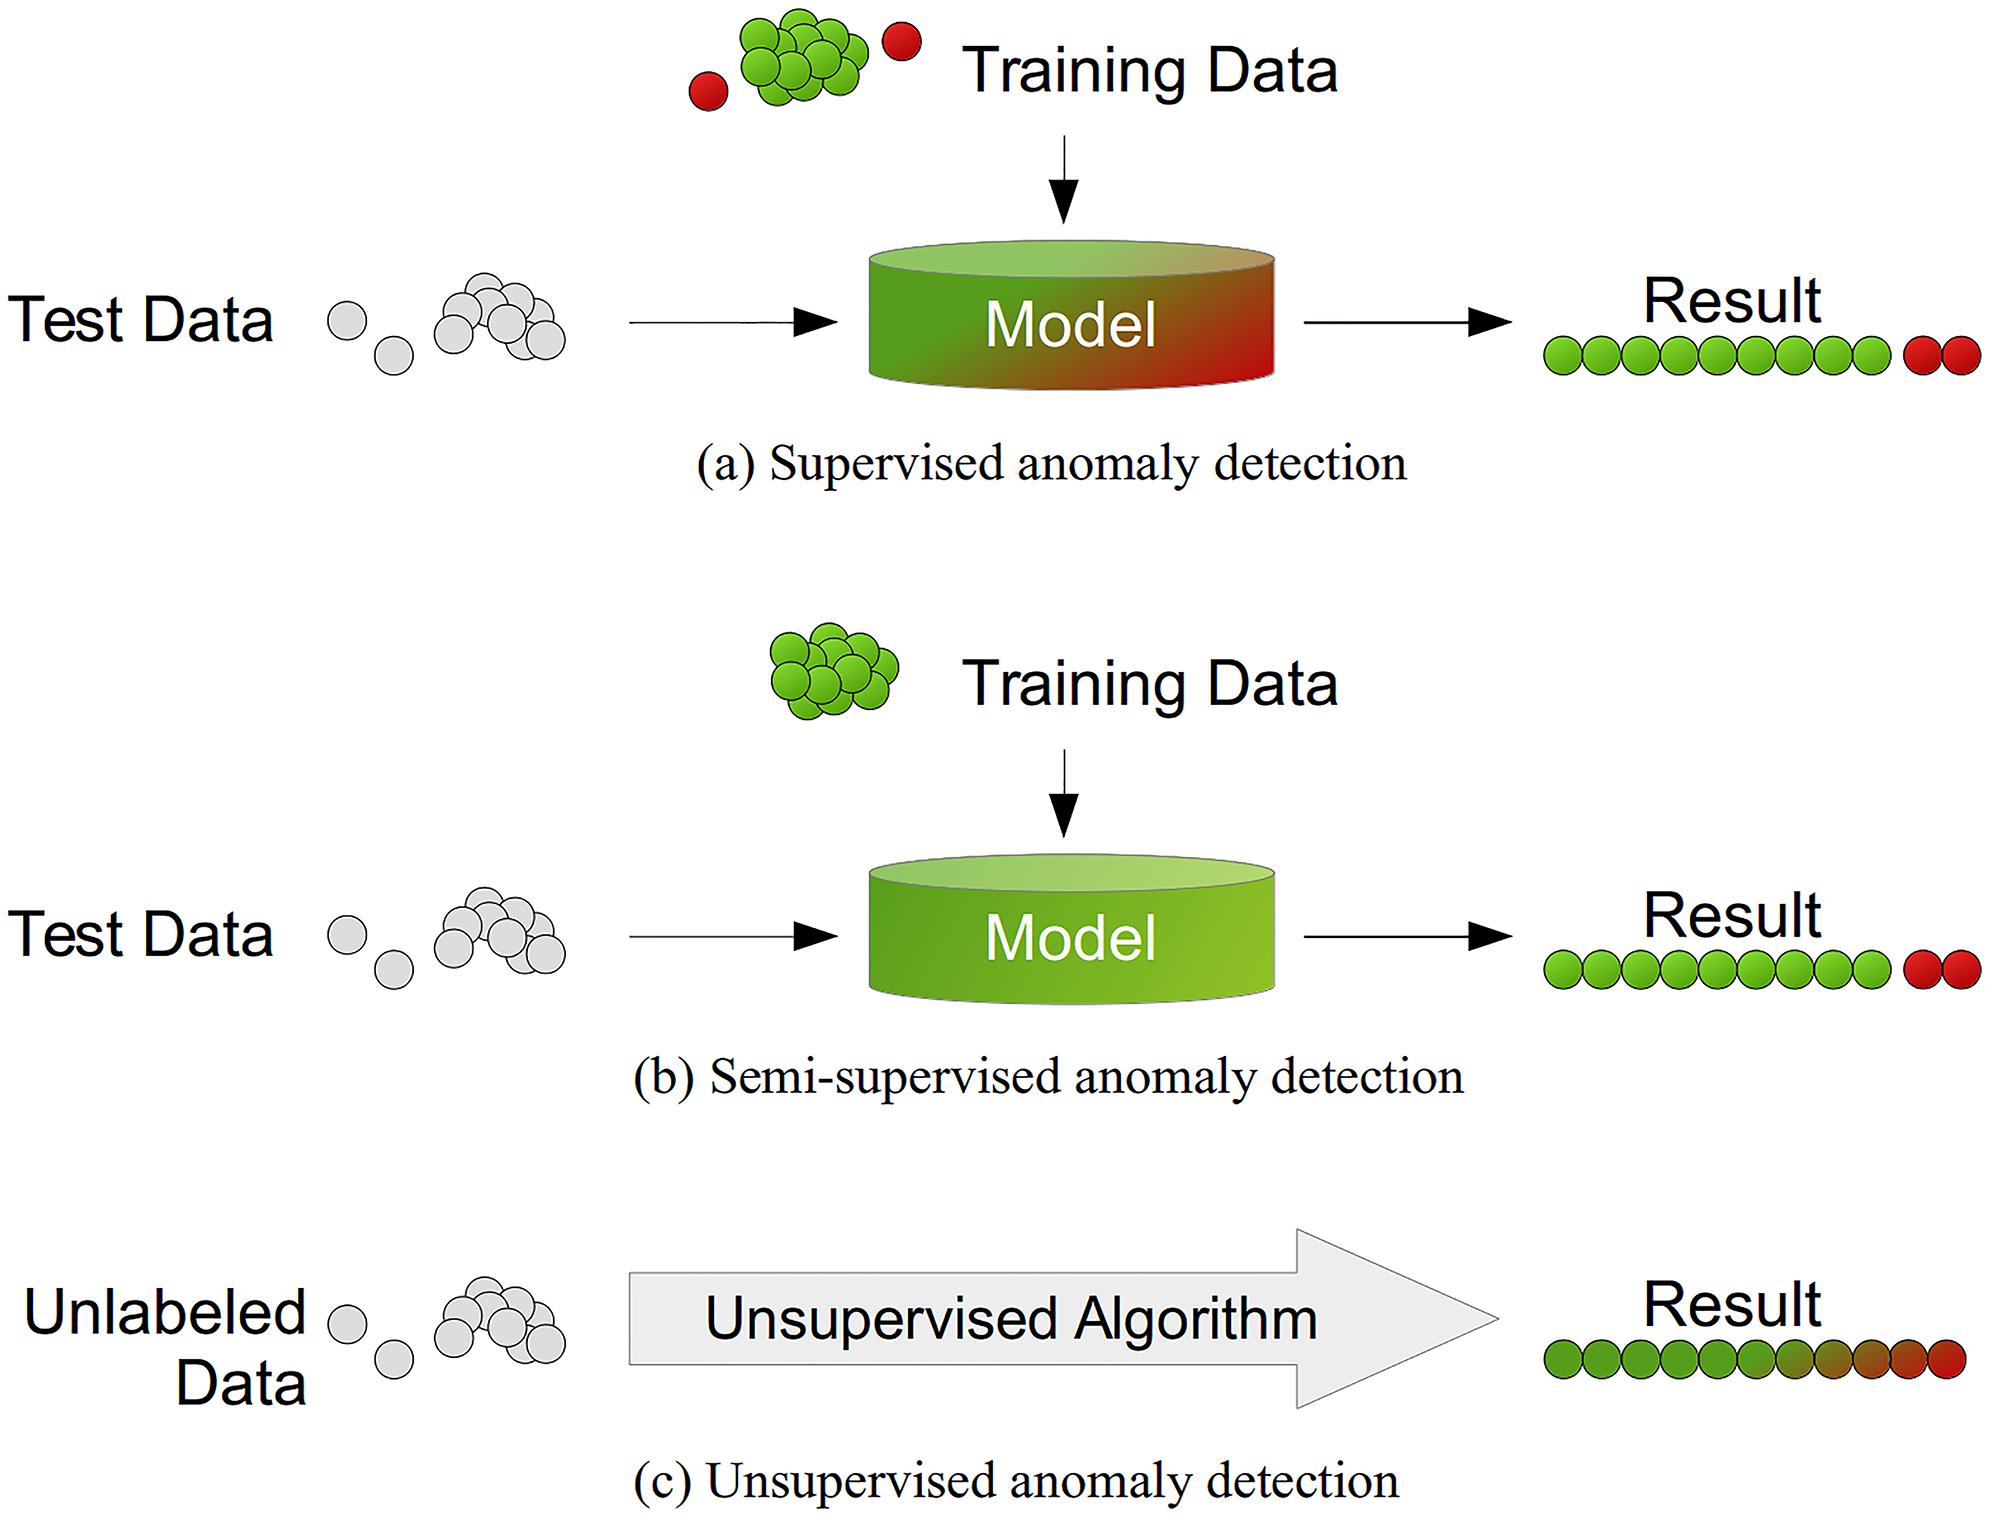
\includegraphics[width=5cm, height =5cm]{./Figures/anomaly.png}
\caption {Anomaly detection approach based on data labels.}
\label{anomaly}
\end{center}
\end{figure}

\end{frame}
%--------------------------------------------------------------------------
\subsection{Data}
\begin{frame}{Data}
\begin{figure}[t!] % "[t!]" placement specifier just for this example
\begin{subfigure}{0.32\textwidth}
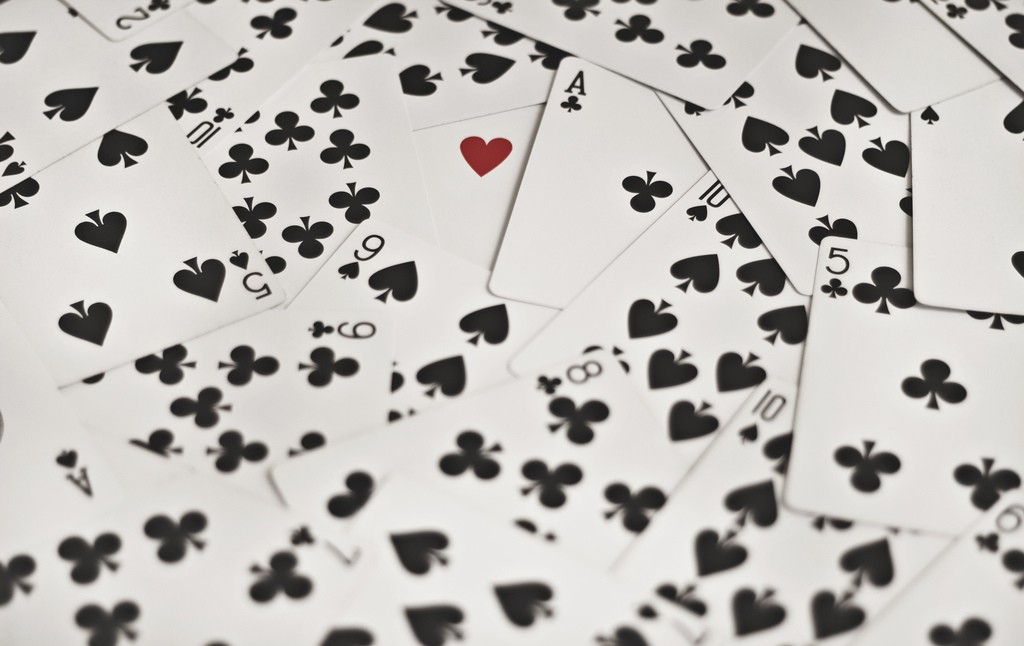
\includegraphics[height=3cm,width=3cm]{./Figures/card.jpg}
\caption{} \label{fig:a}
\end{subfigure}\hspace*{\fill}
\begin{subfigure}{0.32\textwidth}
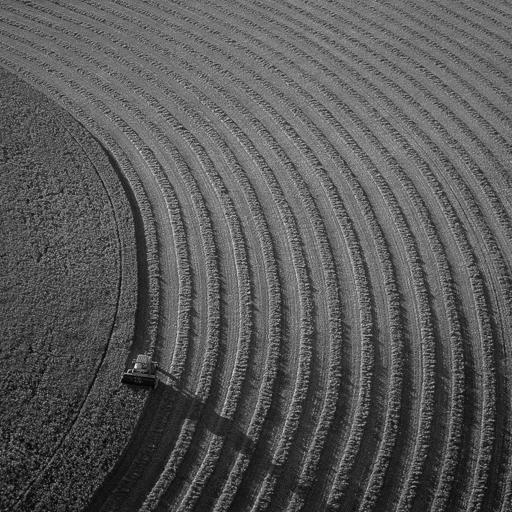
\includegraphics[height=3cm,width=3cm]{./Figures/field.jpg}
\caption{} \label{fig:b}
\end{subfigure}
\begin{subfigure}{0.32\textwidth}
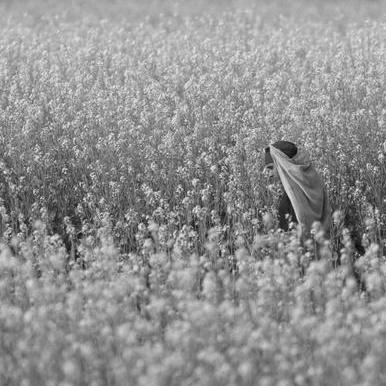
\includegraphics[height=3cm,width=3cm]{./Figures/girl.jpg}
\caption{} \label{fig:c}
\end{subfigure}

\medskip
\begin{subfigure}{0.32\textwidth}
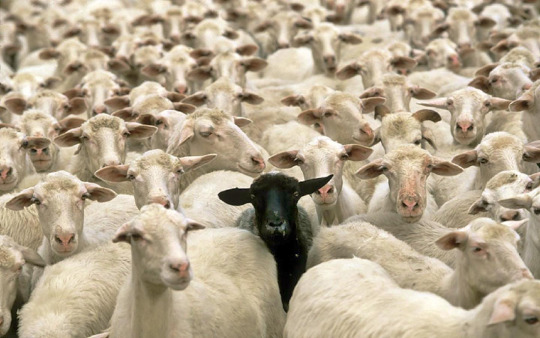
\includegraphics[height=3cm,width=3cm]{./Figures/sheep.jpg}
\caption{} \label{fig:d}
\end{subfigure}\hspace*{\fill}
\begin{subfigure}{0.32\textwidth}
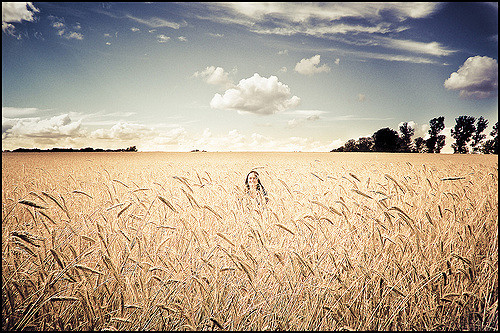
\includegraphics[height=3cm,width=3cm]{./Figures/girlf.jpg}
\caption{} \label{fig:e}
\end{subfigure}
\begin{subfigure}{0.32\textwidth}
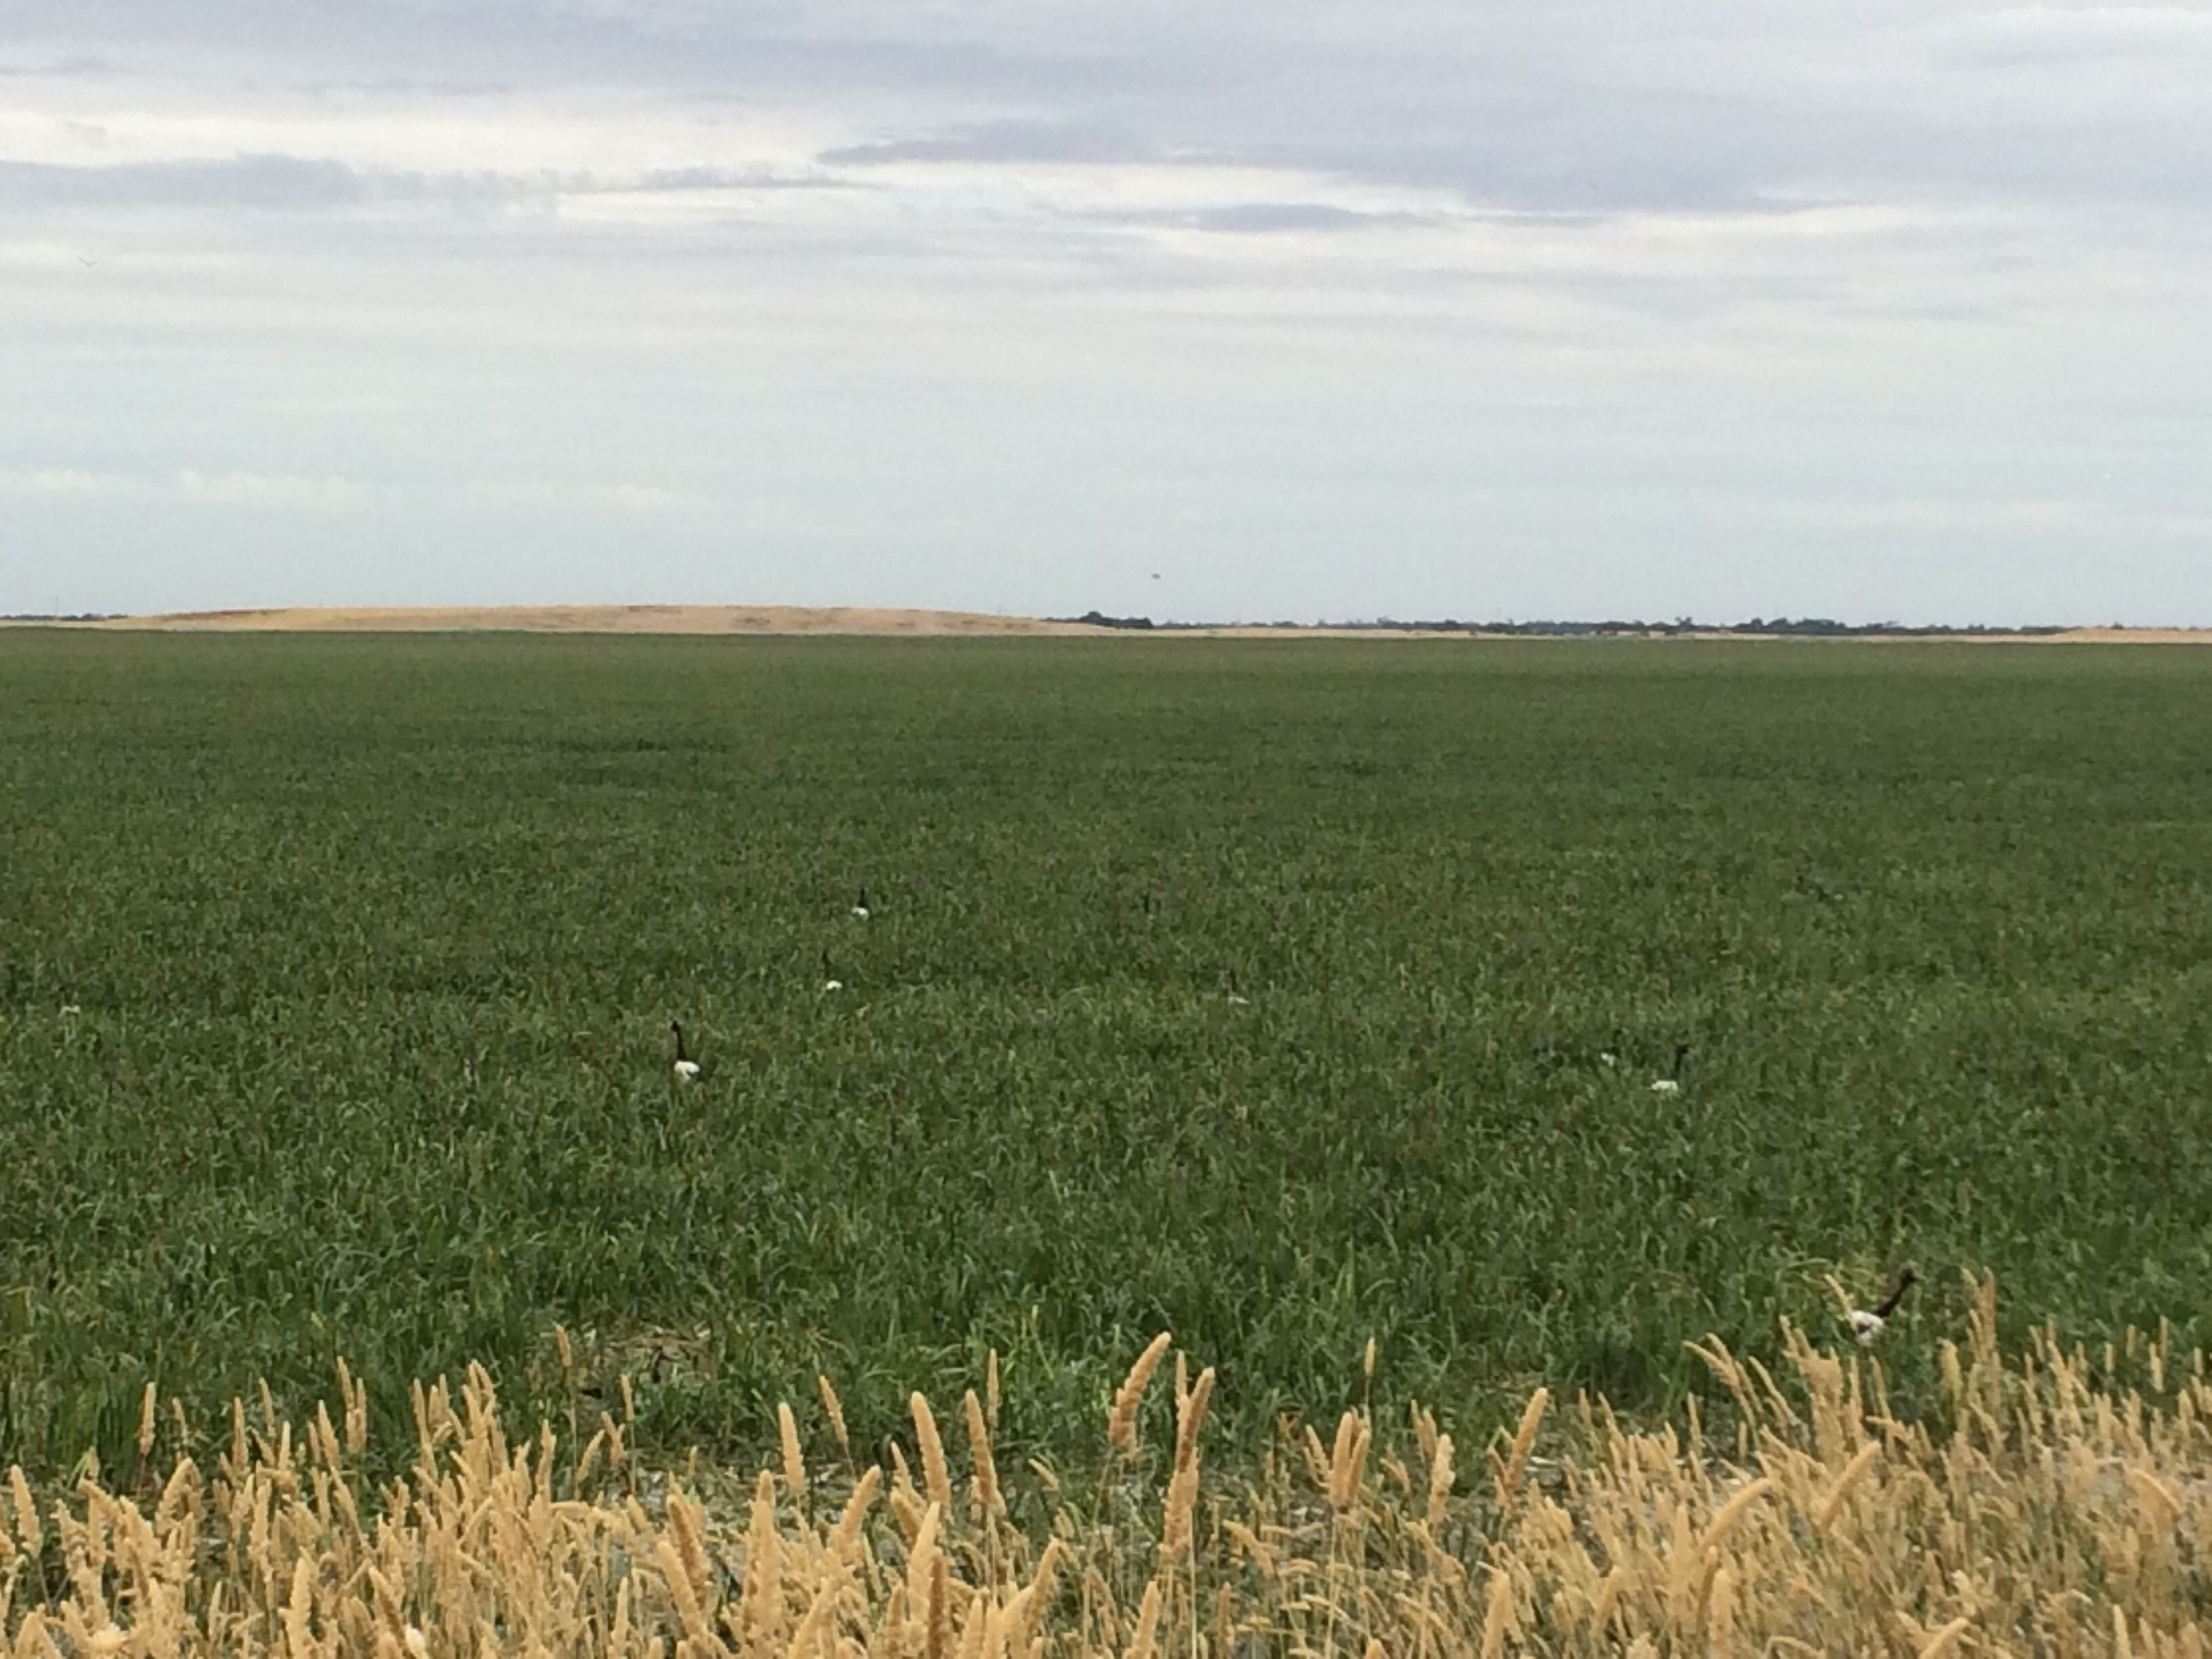
\includegraphics[height=3cm,width=3cm]{./Figures/duck.jpg}
\caption{} \label{fig:f}
\end{subfigure}

\caption{Input Image} \label{fig:input}
\end{figure}
\end{frame}
%--------------------------------------------------------------------------
\subsection{Algorithms}
\begin{frame}{Multiscale Algorithms}
\begin{enumerate}
\item Input Image: $\mathbf{I}$. Size: $400\times400$.
\item For $l = 0:L$ compute Gaussian pyramid $\{\mathbf{G}_{i}\}^{L}_{l=0}$, where $\mathbf{G}_{0}$ is the original image and $\mathbf{G}_{L}$ is the coarsest resolution as discussed in section \ref{C5:LP}.
\item Starting with $\mathbf{G}_L$, sample a subset $\mathbf{I}_{s}$ from $\mathbf{I}$.
\item Compute Diffusion map using $\mathbf{I}_{s}$. 
\item Extend above step to remaining pixels.
\item Calculate anomaly score $\mathbf{C}_l$ for $400\time400$ pixels.
\item Set threshold $\tau_{l}$ to 95th percentile of the anomaly score.
\item If $\mathbf{C}_l > \tau_{l}$, the anomaly will be sampled more densely. Goto step 2, else 
\item output.
\end{enumerate}

\end{frame}
%-------------------------------------------------------------------------
\begin{frame}{Flowchart}
\begin{figure}[ht]
\begin{center}
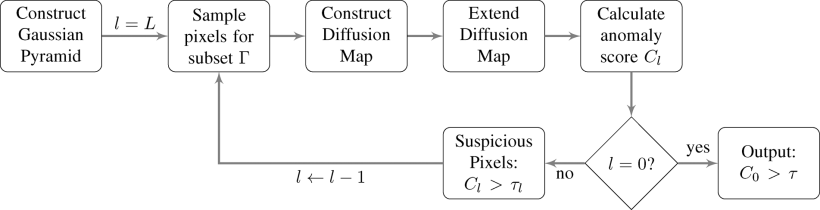
\includegraphics[width=\textwidth]{./Figures/algo.png}
\caption {Multiscale Algorithm.}
\label{algo}
\end{center}
\end{figure}

\end{frame}
%--------------------------------------------------------------------------

%--------------------------------------------------------------------------
\subsection{Results}
\begin{frame}{Results: True Positive (Basic)}

\begin{figure}[ht]
\begin{center}
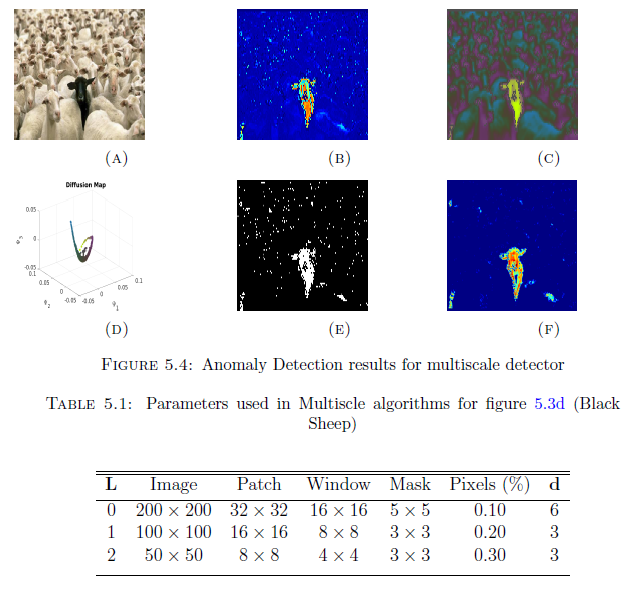
\includegraphics[width=8cm, height =8cm]{./figures/R_1.png}
\label{algo}
\end{center}
\end{figure}

\end{frame}
%--------------------------------------------------------------------------
\begin{frame}{Results: True Positive (Complex)}

\begin{figure}[ht]
\begin{center}
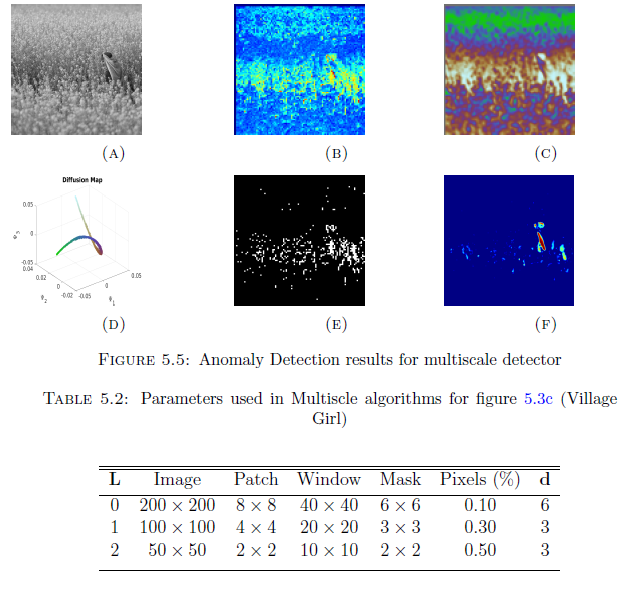
\includegraphics[width=8cm, height =8cm]{./figures/R_2.png}
\label{algo}
\end{center}
\end{figure}

\end{frame}

%--------------------------------------------------------------------------
\begin{frame}{Results: False Alarm (Complex)}

\begin{figure}[ht]
\begin{center}
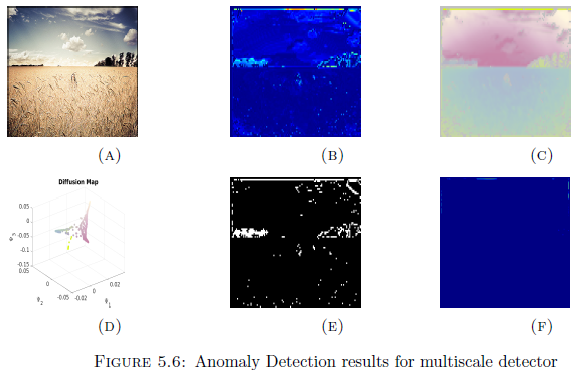
\includegraphics[width=8cm, height =4cm]{./figures/R_3.png}
\label{algo}
\end{center}
\end{figure}
\begin{figure}[ht]
\begin{center}
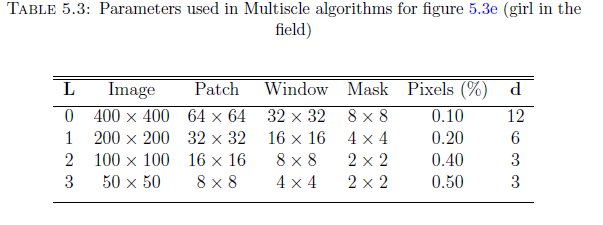
\includegraphics[width=8cm, height =3cm]{./figures/R_4.png}
\label{algo}
\end{center}
\end{figure}

\end{frame}
%--------------------------------------------------------------------------
\section{Conclusions}

\begin{frame}{Conclusions}

\begin{enumerate}
\item Deviating from primary evaluation methodology of manifold leaning algorithms based on artificial data sets, we use MNIST datasets with optical character recognition in mind.
\item The out of sample prediction for manifold algorithms indicates that test points are projected on the corrects clusters of training datasets, but separation of some numbers were blurred.
\item The preprocessing of MNIST data by manifold learning algorithms didn't improve accuracy in optical character recognition. 
\item The proposed algorithms performs well the images which is not too contrast, but gives false positive on image which is of high resolutions.
\end{enumerate}

\end{frame}
%--------------------------------------------------------------------------
\begin{frame}{Future Work}
\begin{enumerate}
\item When answering the questions on evaluating the results of manifold learning, we need to take in account of manifold structure and noises.
\item When there is multiple sub-manifolds of possibly different dimensionalities embedded in high dimensional complex data, it is most unlikely that the existing manifold learning approaches can discover all the interesting lower-dimensional structures. There is need to develop a hierarchical manifolds learning framework to discover a variety of the underlying low dimensional structures.
\item In optical character recognition, there is need to optimize the model when calculating accuracy. 
\item A future extension of this work would be combine  anomaly scores from the different multiscale levels into a single anomaly score. This will enable detecting anomalies of different size in an image, which this algorithms fails to address.
\end{enumerate}

\end{frame}
%--------------------------------------------------------------------------
\begin{frame}
\Huge{\centerline{Questions?}}
\end{frame}

%----------------------------------------------------------------------------------------

\end{document} 